%!TEX root = ../hbrs-poster.tex
\documentclass[hbrs-poster.tex]{subfiles}
\begin{document}
    \block{Results}
    {
    The metrics used to evaluate the deep learning (DL) classifier are mean average precision, F1 score and Jaccard score. The DL model achieved the highest scores indicating superior performance in predicting movie genres.
        \begin{tikzfigure}
                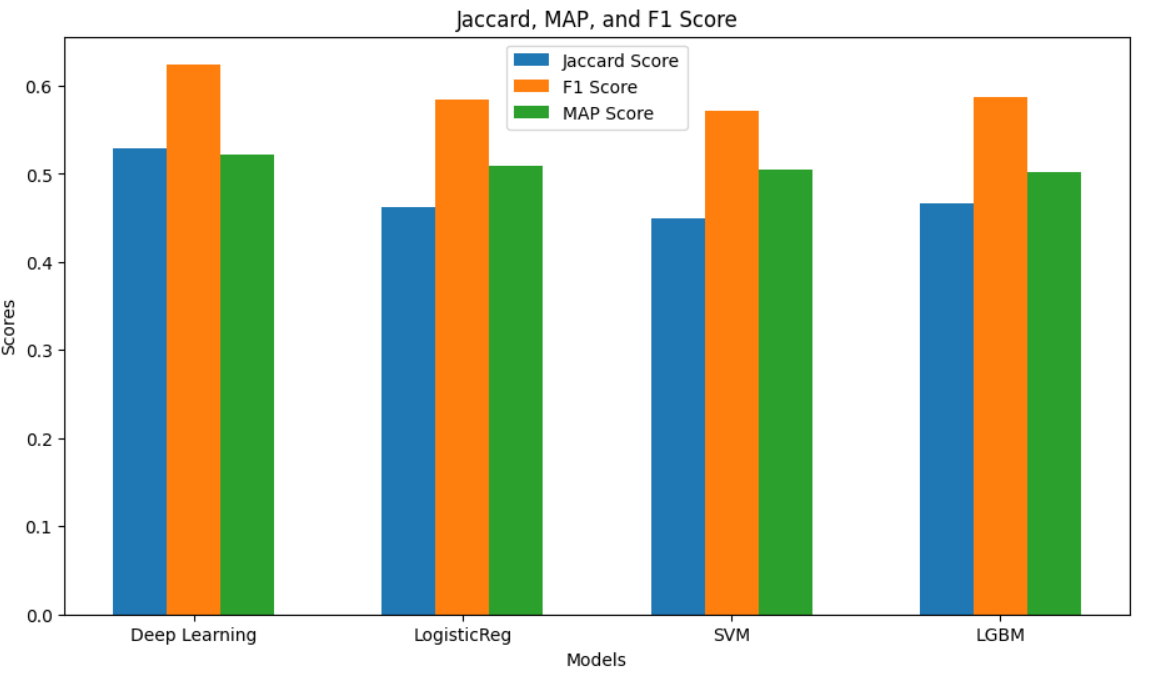
\includegraphics[width=0.325\textwidth, height=0.1\textheight]{figures/metrics.png}
            \end{tikzfigure}

    The below confusion matrix for our DL model indicates that most of the predictions made are correct and it gives an intuition of how the classifier understands the plot summaries and which genres does it confuse with for each genre.
    \begin{tikzfigure}
                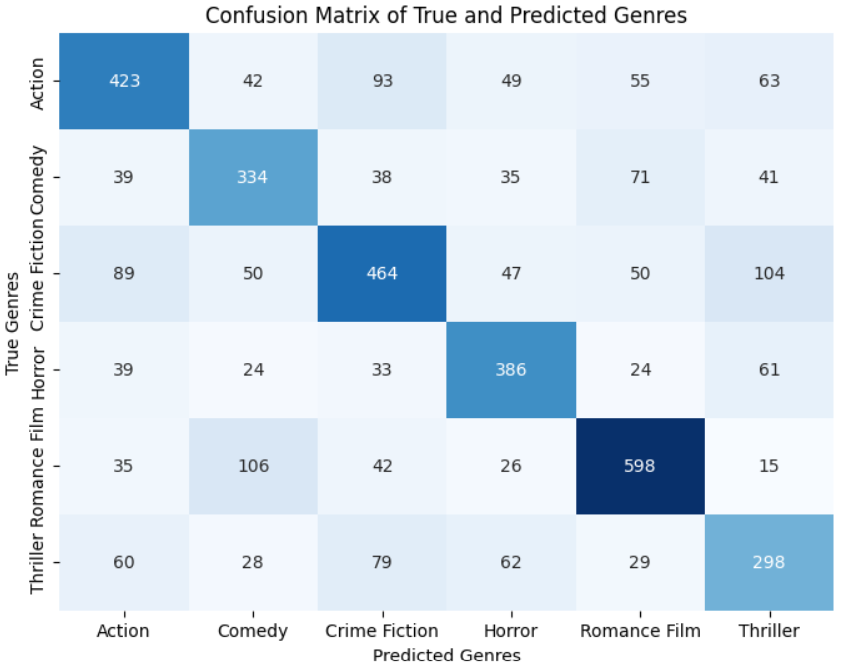
\includegraphics[width=0.325\textwidth, height=0.1\textheight]{figures/confusion_matrix.png}
    \end{tikzfigure}
    }
\end{document}
